%% NEED FURTHER INTRODUCTION
The first infinite matter system we will analyze with the SRE method is the homogeneous electron gas (HEG), described in Chapter 4. The HEG, as one of the simpler infinite matter systems, is an excellent sandbox to fully develop the SRE method described in the last chapter.



Fig. \ref{increase_m} shows the results of computing the CCD correlation per energy for a HEG with $r_s$ = 0.5 at various numbers of electrons and with four different numbers of single-particle states. We can see that the calculation of $\Delta E_{CC}$ depends heavily on the number of single-particle states in the system, and we can begin to see that the correlation energy converges as the number of single-particle states in the system increases. The calculations performed with only 514 single-particle states (or 15 shells) are the least accurate of the four plots in Fig. \ref{increase_m} since they are performed with the fewest single-particle states. On the other hand, the calculations performed with 6,142 single-particle states (or 70 shells in total) are the most accurate of the four plots, and in fact, the convergence of $\Delta E_{CC}$ has been confirmed at this point. However, it is not always feasible to perform the calculations at this high number of single-particle states due to the associated high computational time and resource requirements.

\begin{figure}
    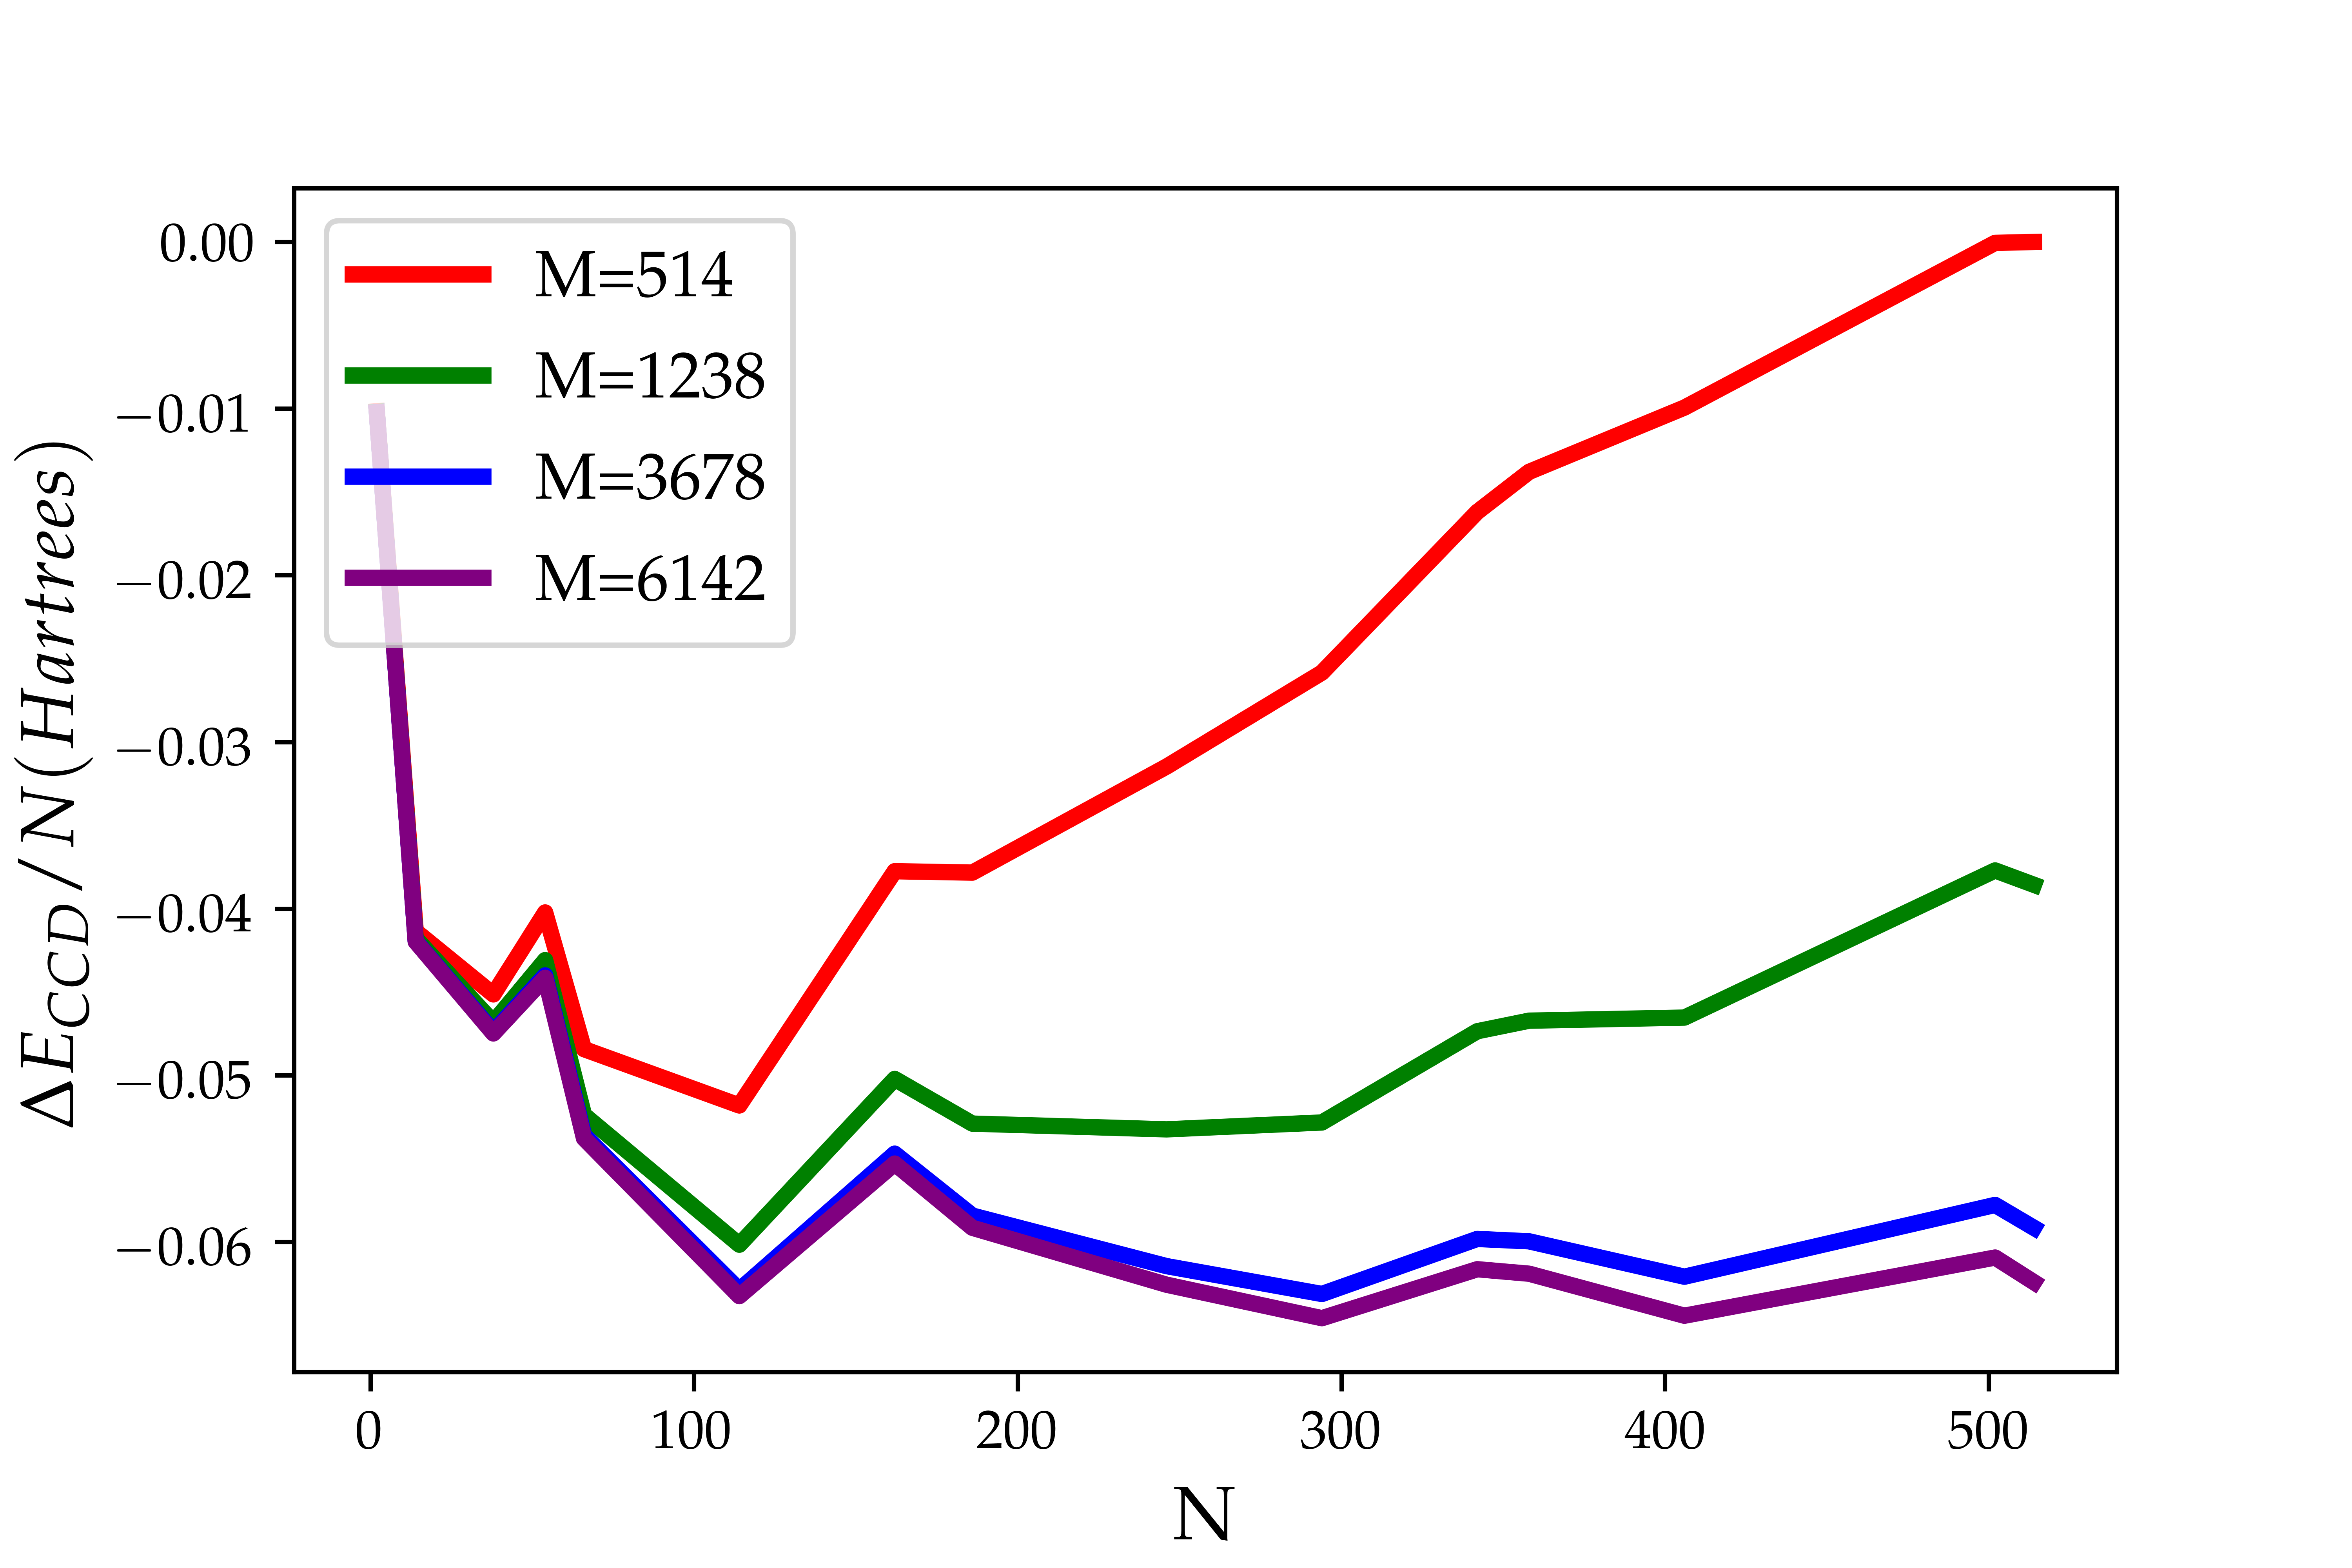
\includegraphics[scale=0.75]{Images/Chapter7/ElectronGas/Increase_M.png}
    \captionof{figure}{$\Delta E_{CC}$ per electron plotted against N with calculations performed at four different values of M. As M increases, the error in the calculation decreases, but the run time drastically increases.}
    \label{increase_m}
\end{figure}

Fig. \ref{fig:EG_times} shows the total run time in node seconds for CCD calculations of the HEG with $r_s$ = 0.5, N = 66, 294, or 514, and at various numbers of single-particle states. Node seconds will be used to report computational run times in this thesis such that run times generated with different numbers of MPI nodes can be compared. A \textit{node second} is defined as the run time of the coupled cluster program (in seconds) times the number of MPI nodes used in the calculation. For the HEG, all calculations were performed using nodes from Michigan State University's high-performance computing center. Each node is an Intel Xeon processor with a reported clock speed of 2.4 GHz. Each coupled cluster program was run with four MPI nodes and 28 OpenMP threads. The specifications of the coupled cluster code used to perform the HEG and neutron matter calculations with the Minnesota potential shown in the section are described in Ref. \cite{Ref5}.

In Fig. \ref{fig:EG_times}, there is a consistent pattern in the data where more electrons and more single-particle states in a calculation require a longer run time. This is an obvious and expected result, and in fact, the CCD run times should scale polynomially with the number of particles and single particle states allowed in the calculation. For example, a CCD calculation of the HEG should scale as $O(N^4M^6)$, where typically M >> N \cite{Ref2}. If we look at the results for N = 66 and assume that the converged CCD correlation energy occurs at M = 6,142 single-particle states (see Fig. \ref{increase_m}), the total run time for the CCD program is 653.88 node seconds (10.89 node minutes). However, generating the converged CCD correlation energy for N = 514 and M = 6,142 takes 42791.75 node seconds (11.88 \textbf{node hours}). Thus while generating the converged CCD correlation energies at a smaller number of particles results in possible computational run times, performing the same calculation at a large number of electrons is not feasible in most studies.

\begin{figure}
    \centering
    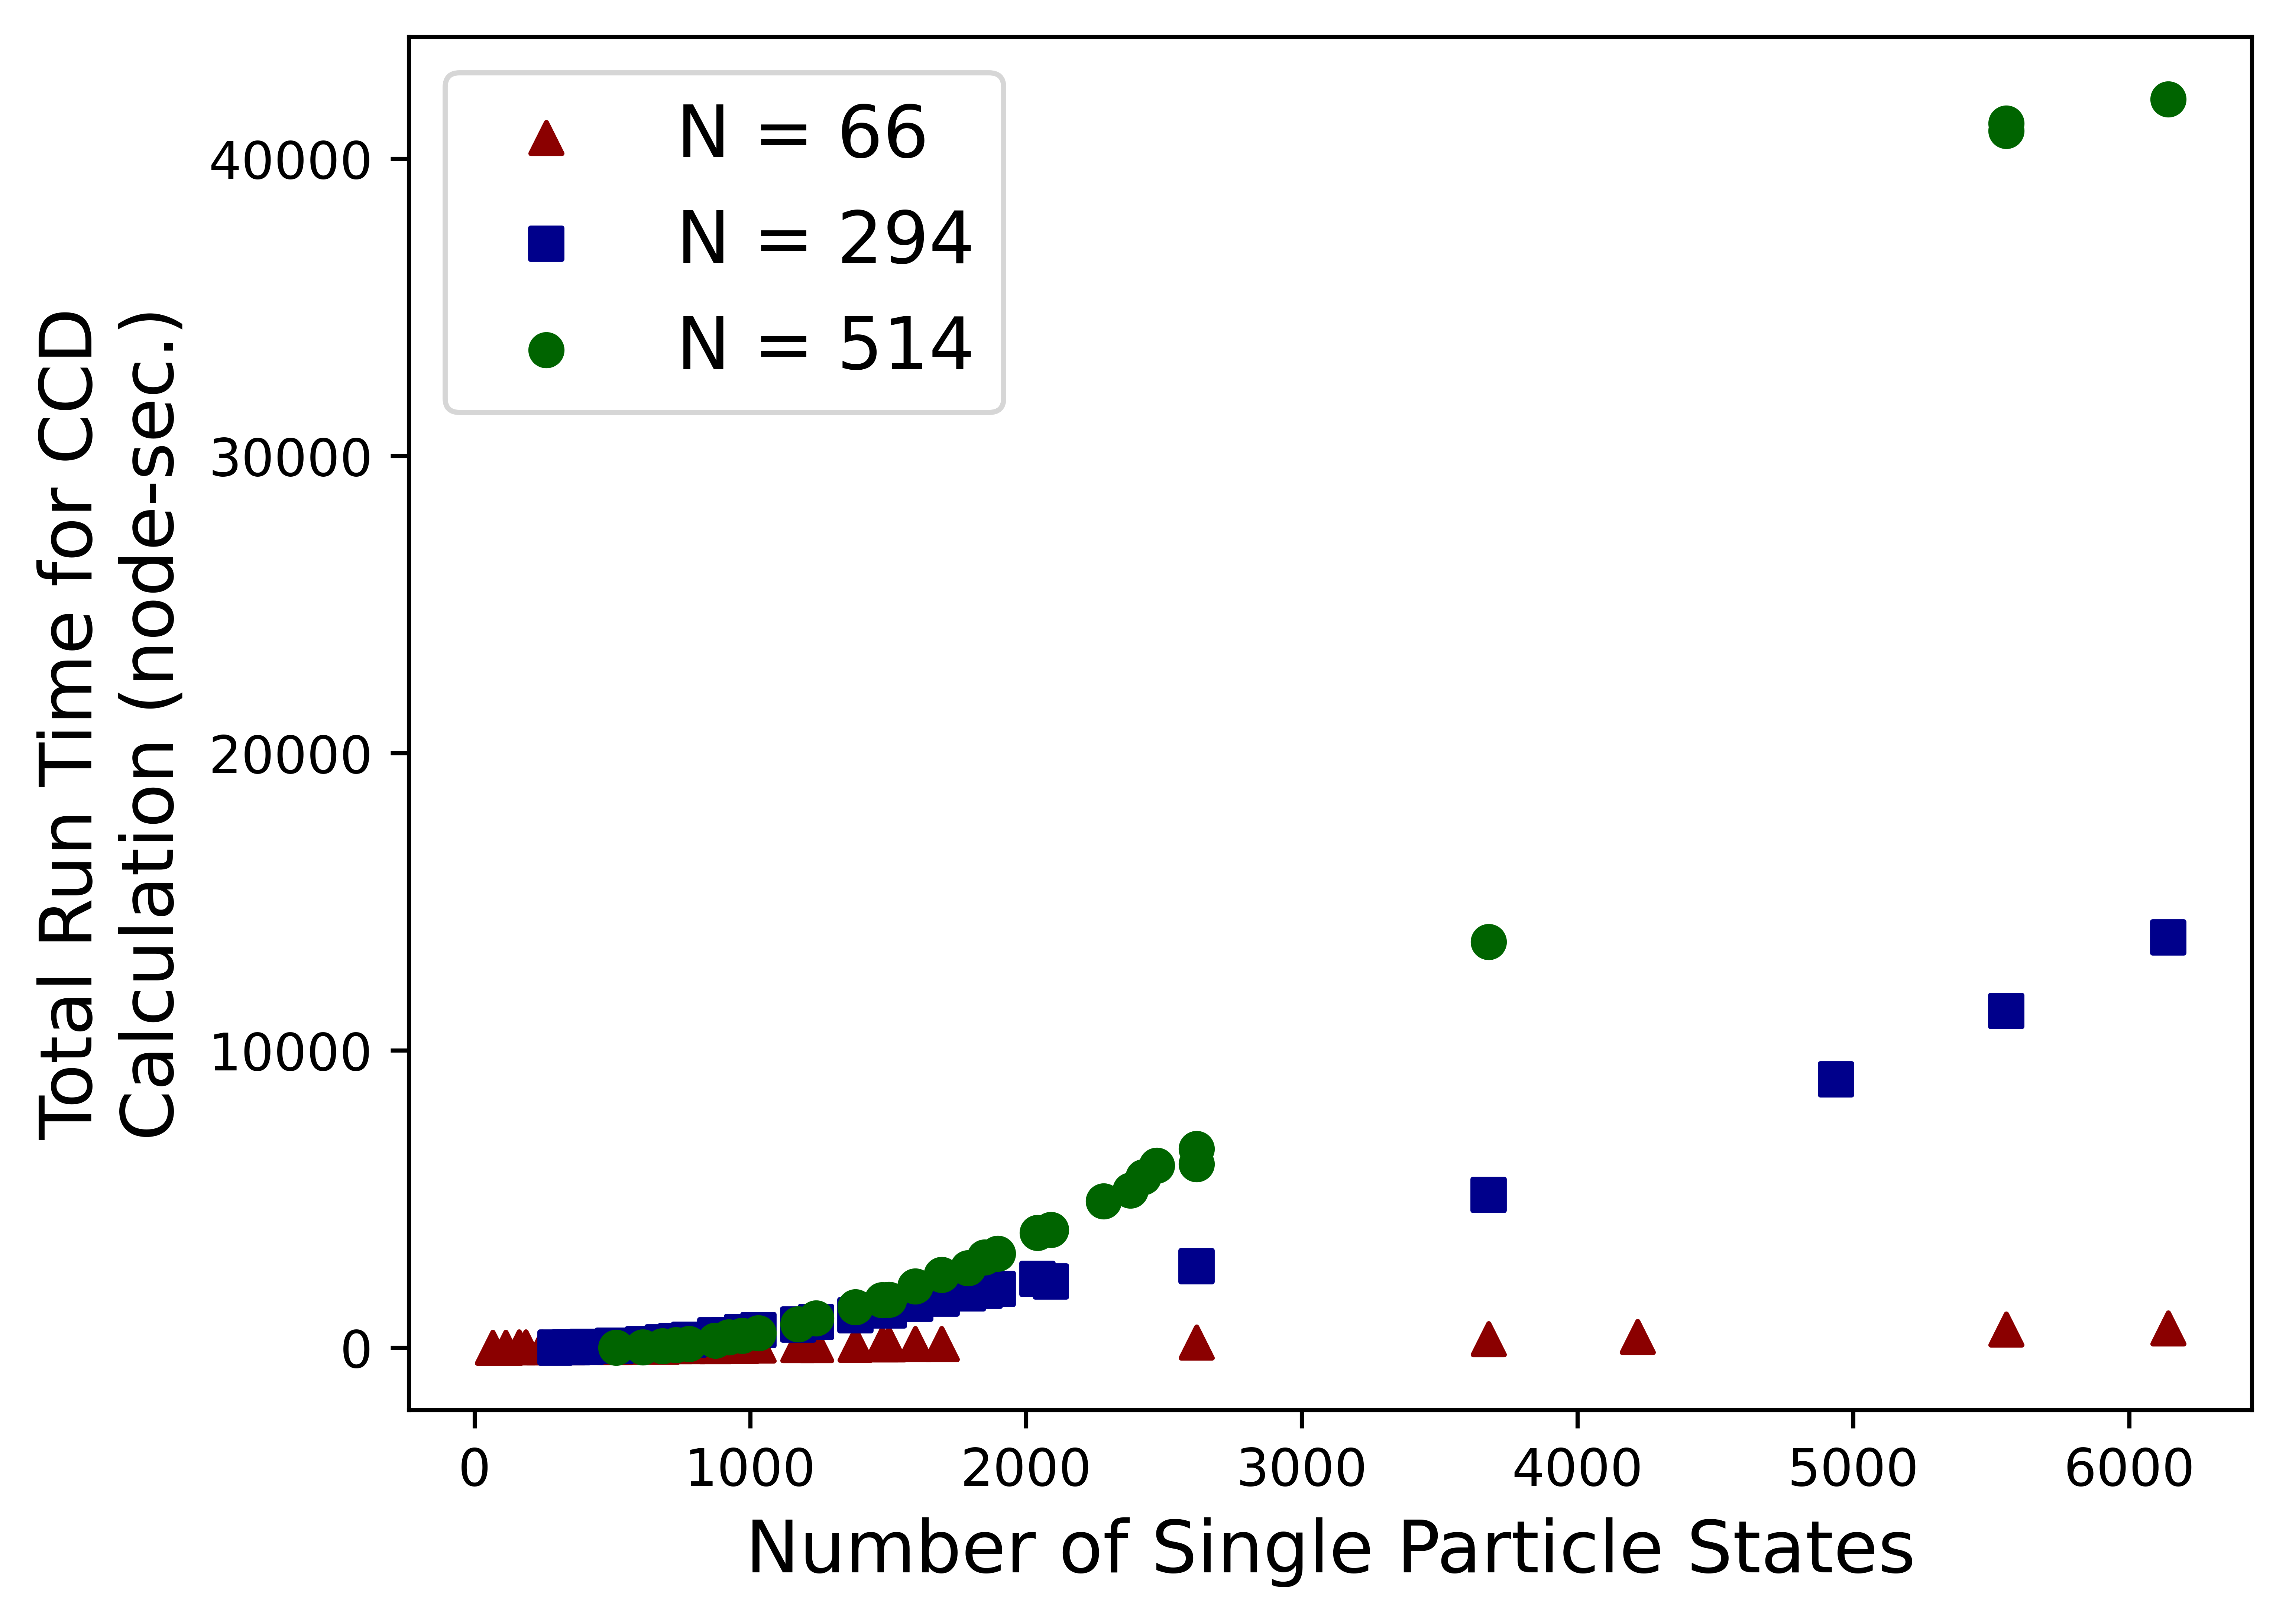
\includegraphics[scale=0.75]{Images/Chapter7/ElectronGas/EG_timing_graph_node_sec.png}
    \caption{The total run time needed, in node seconds, to perform a CCD calculation on the HEG with $r_s$ = 0.5 and at N = 66, 294, and 514. The CCD calculations are performed at many values of M, as shown on the x-axis. A node second is defined as the total run time of the program times the number of nodes used to run the program. Four nodes from Michigan State University's high-performance supercomputer were utilized in this case. These nodes have Intel Xeon processes with a clock speed of 2.4 GHz.}
    \label{fig:EG_times}
\end{figure}

Another factor we can look at is the amount of RAM needed to perform the CCD calculations at various numbers of electrons and single-particle states. The amount of RAM needed to perform the calculations should increase as both N and M increase as, naively, the Hamilton for the system should be ${MN}\choose{N}$ on each side. However, modern advancements limit the number of matrix elements that must be computed and stored. Fig. \ref{fig:eg_ram} shows the total amount of RAM (in gigabytes) needed to perform CCD calculations for the HEG at $r_s$ = 0.5. There are three different numbers of electrons represented in the figure: N = 66 (red triangles), N = 294 (blue squares), and N = 514 (green circles). These numbers of electrons span the range of interest for this work. The number of single-particle states varied from less than 1,000 to over 6,000. We see a consistent pattern in the data where the amount of RAM needed for the calculation increases as the number of electrons and single-particle states changes. The converged CCD correlation energy for 514 electrons (the highest amount of electrons in this thesis) and at 6,142 single particle states takes a startling 283.79 GB of RAM to run. However, the converged CCD correlation energy at 66 electrons and 6,142 single particle states still takes 106.49 GB of RAM, a very moderate number of particles to have in a calculation. Therefore, not only is computing the converged CCD correlation energies expensive in the amount of computational time required, but the converged correlation energies also take a considerable amount of computational resources, requiring a supercomputer for these calculations to be feasible.

\begin{figure}
    \centering
    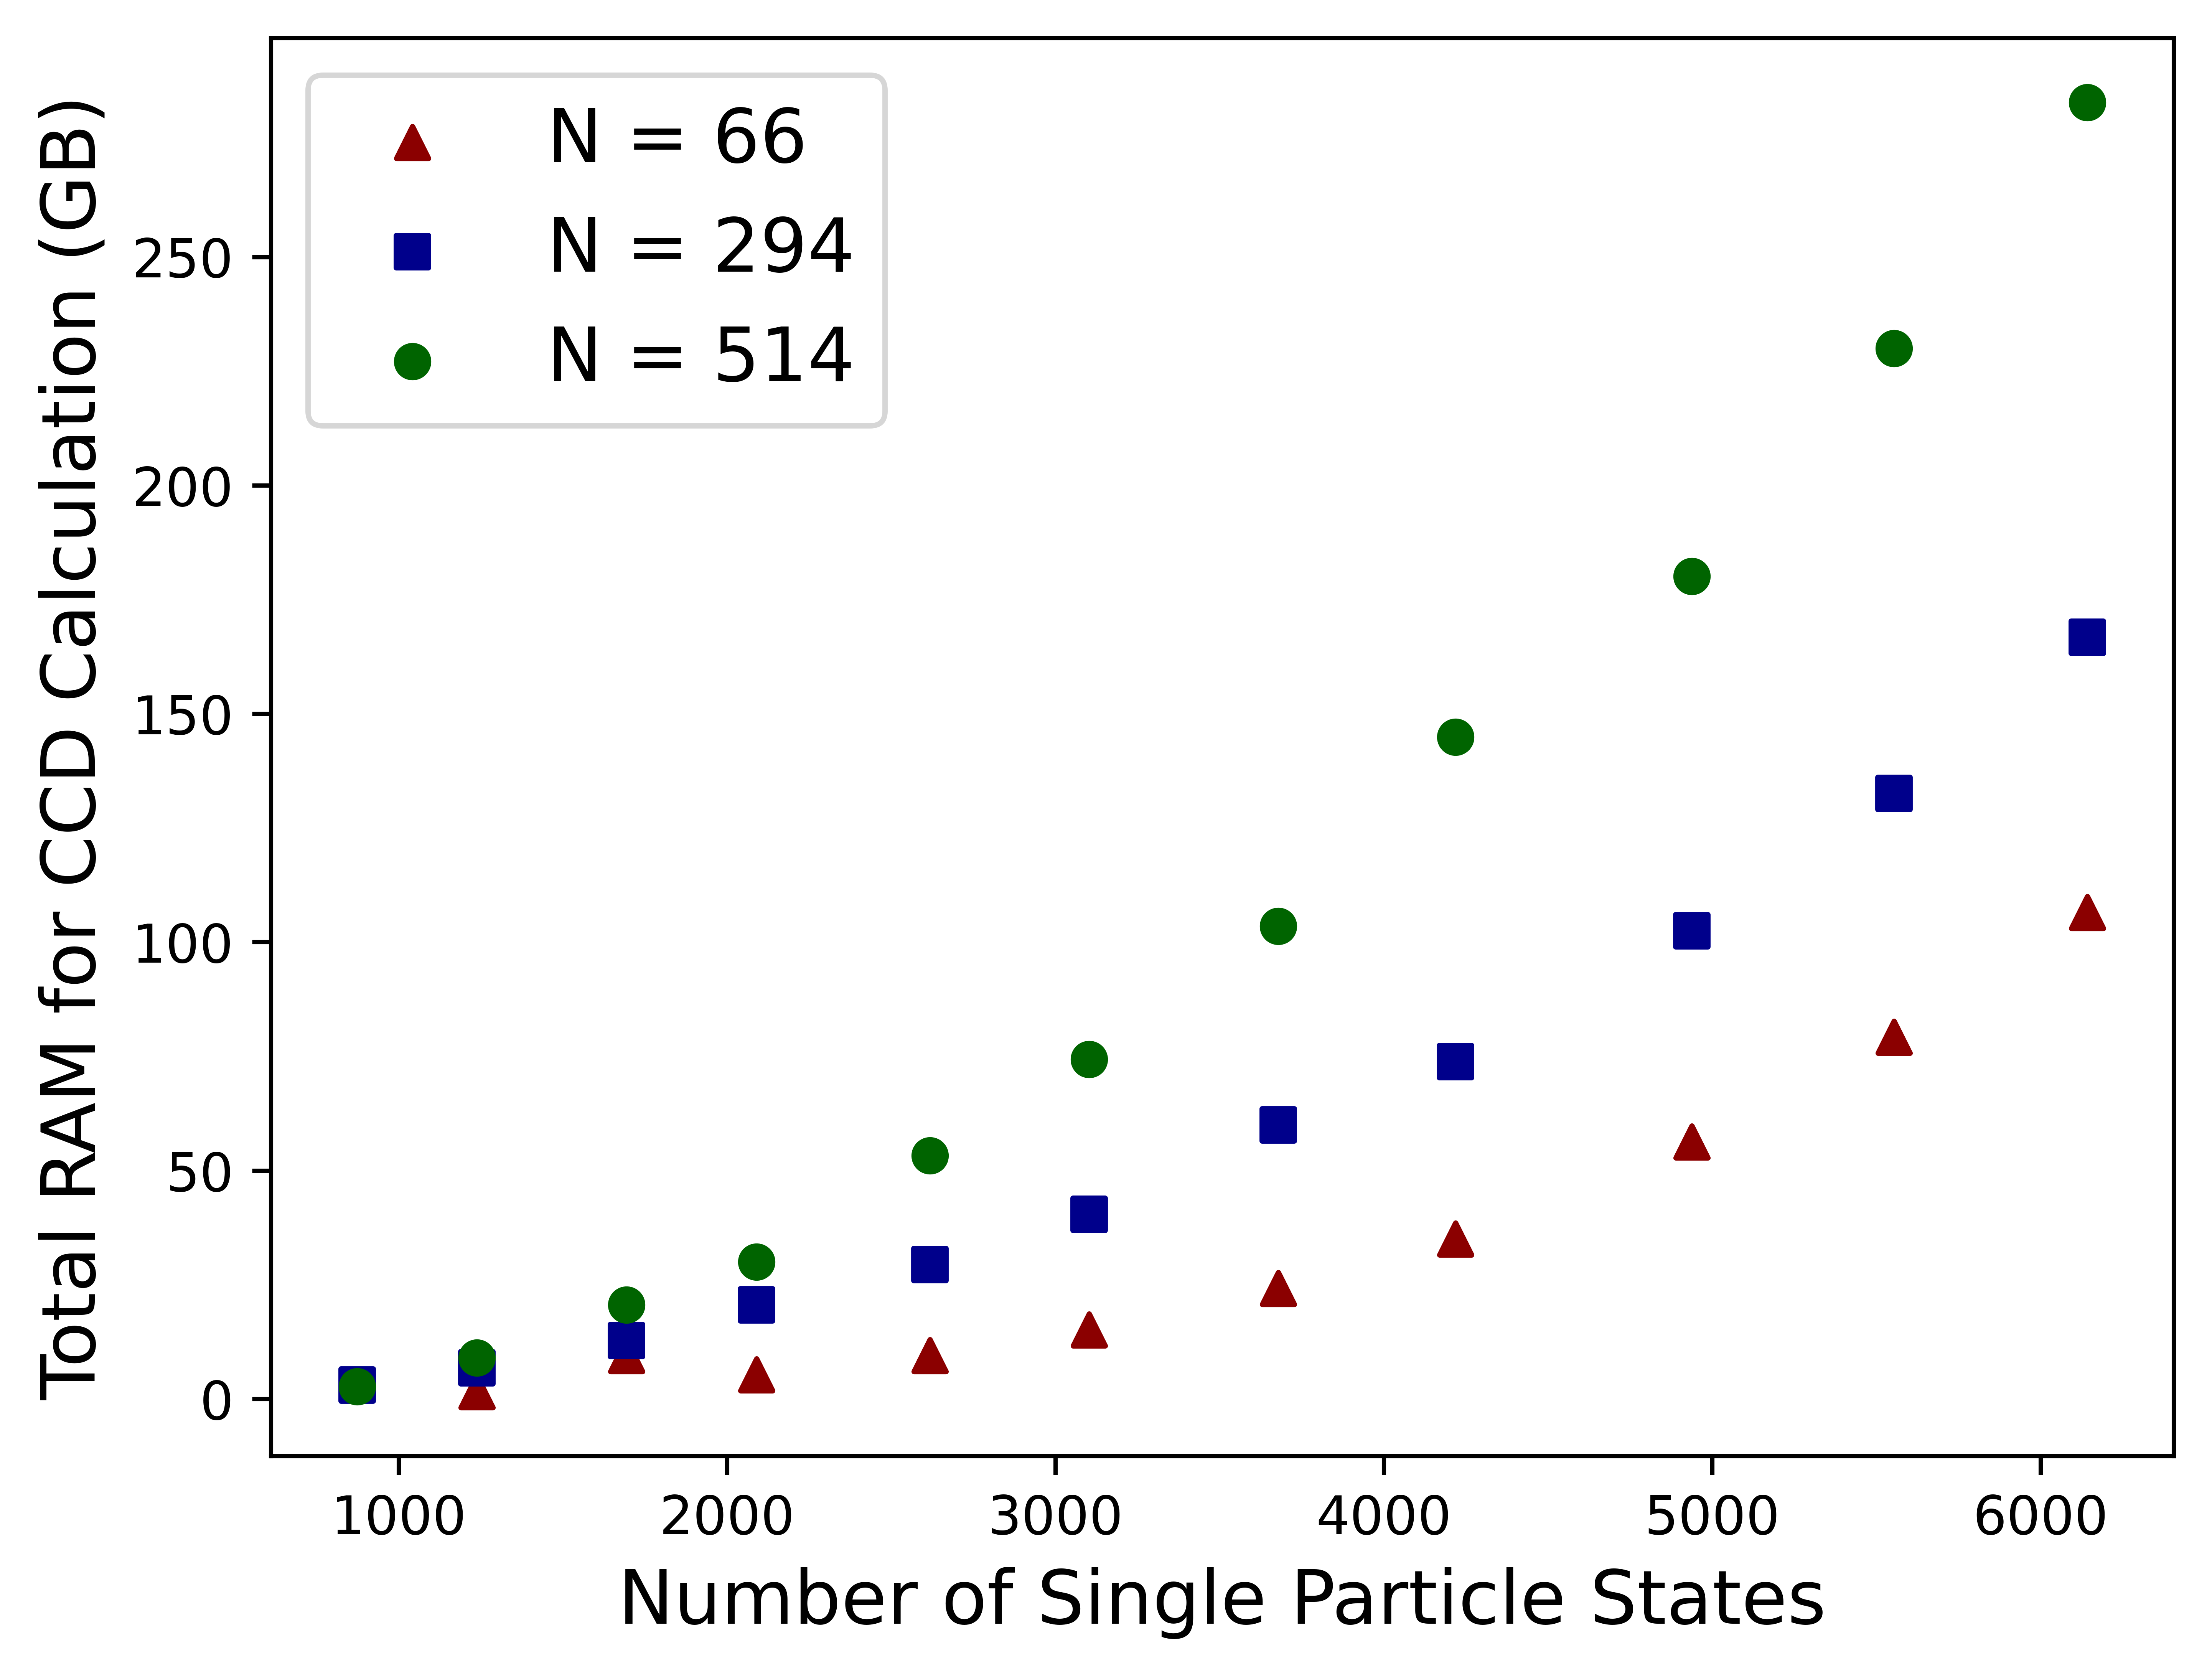
\includegraphics[scale=0.75]{Images/Chapter7/EG_RAM.png}
    \caption{The total amount of RAM in gigabytes needed to perform CCD calculations on the HEG with $r_s$ = 0.5 and with 66, 294, or 514 electrons.  Calculations were performed at various numbers of single-particle states (x-axis).}
    \label{fig:eg_ram}
\end{figure}

%% COMPLETE THE MOTIVATION HERE 
Thus, though increasing the number of single-particle states in a CCD calculation of the HEG increases the accuracy of the CCD correlation energy, it comes with high computational time and resource considerations that can make these calculations infeasible. Therefore, we are motivated to develop a method by which the CCD correlation energies at a high number of single-particle states can be recreated using only calculations performed at a lower number of single-particle states, where the computational resource and time requirements are significantly more reasonable.

In Fig. \ref{mbpt_and_cc}, $\Delta E_{CCD}$ and $\Delta E_{MBPT2}$ is plotted as a function of the number of single-particle states in the calculation for a HEG system with $r_s$ = 0.5 and 342 electrons. The CCD results are plotted in red, and the MBPT results are in blue. The calculations up to 2,090 single-particle states are plotted with the solid lines, and then the converged correlation energies are plotted with the dashed lines. It is much easier in this figure to see that the correlation energies converge as the number of single-particle states increases and that even at around 2,000 single-particle states, the correlation energies are not close to their converged values. However, the ranges of single-particle states shown in this figure with the solid lines are the calculations we wish to use to predict the converged CCD correlation energy, as at these ranges, the computational time and resource requirements are reasonable.

There are a few important things to note in Fig. \ref{mbpt_and_cc}.  First, there is a significant difference between the converged correlation energies, meaning that even though it is easier to generate $\Delta E_{MBPT}$ compared to $\Delta E_{CC}$, $\Delta E_{MBPT}$ is not a good approximation to the true correlation energy. Second, though it takes 21,735.10 node seconds (6.03 node hours) to calculate $\Delta E_{CC,6142}^{342}$ it only takes 5.12 node seconds to generate $\Delta E_{MBPT,6142}^{342}$.  Thus generating the converged MBPT2 correlation energies is significantly faster than generating the converged CCD correlation energies. The MBPT2 calculations are faster by four orders of magnitude. Finally, note that though the MBPT2 and CCD calculations converge to different values, they converge at roughly the same rate and display similar patterns in their convergence. This similarity in convergence was the inspiration for the SRE method.

\begin{figure}
    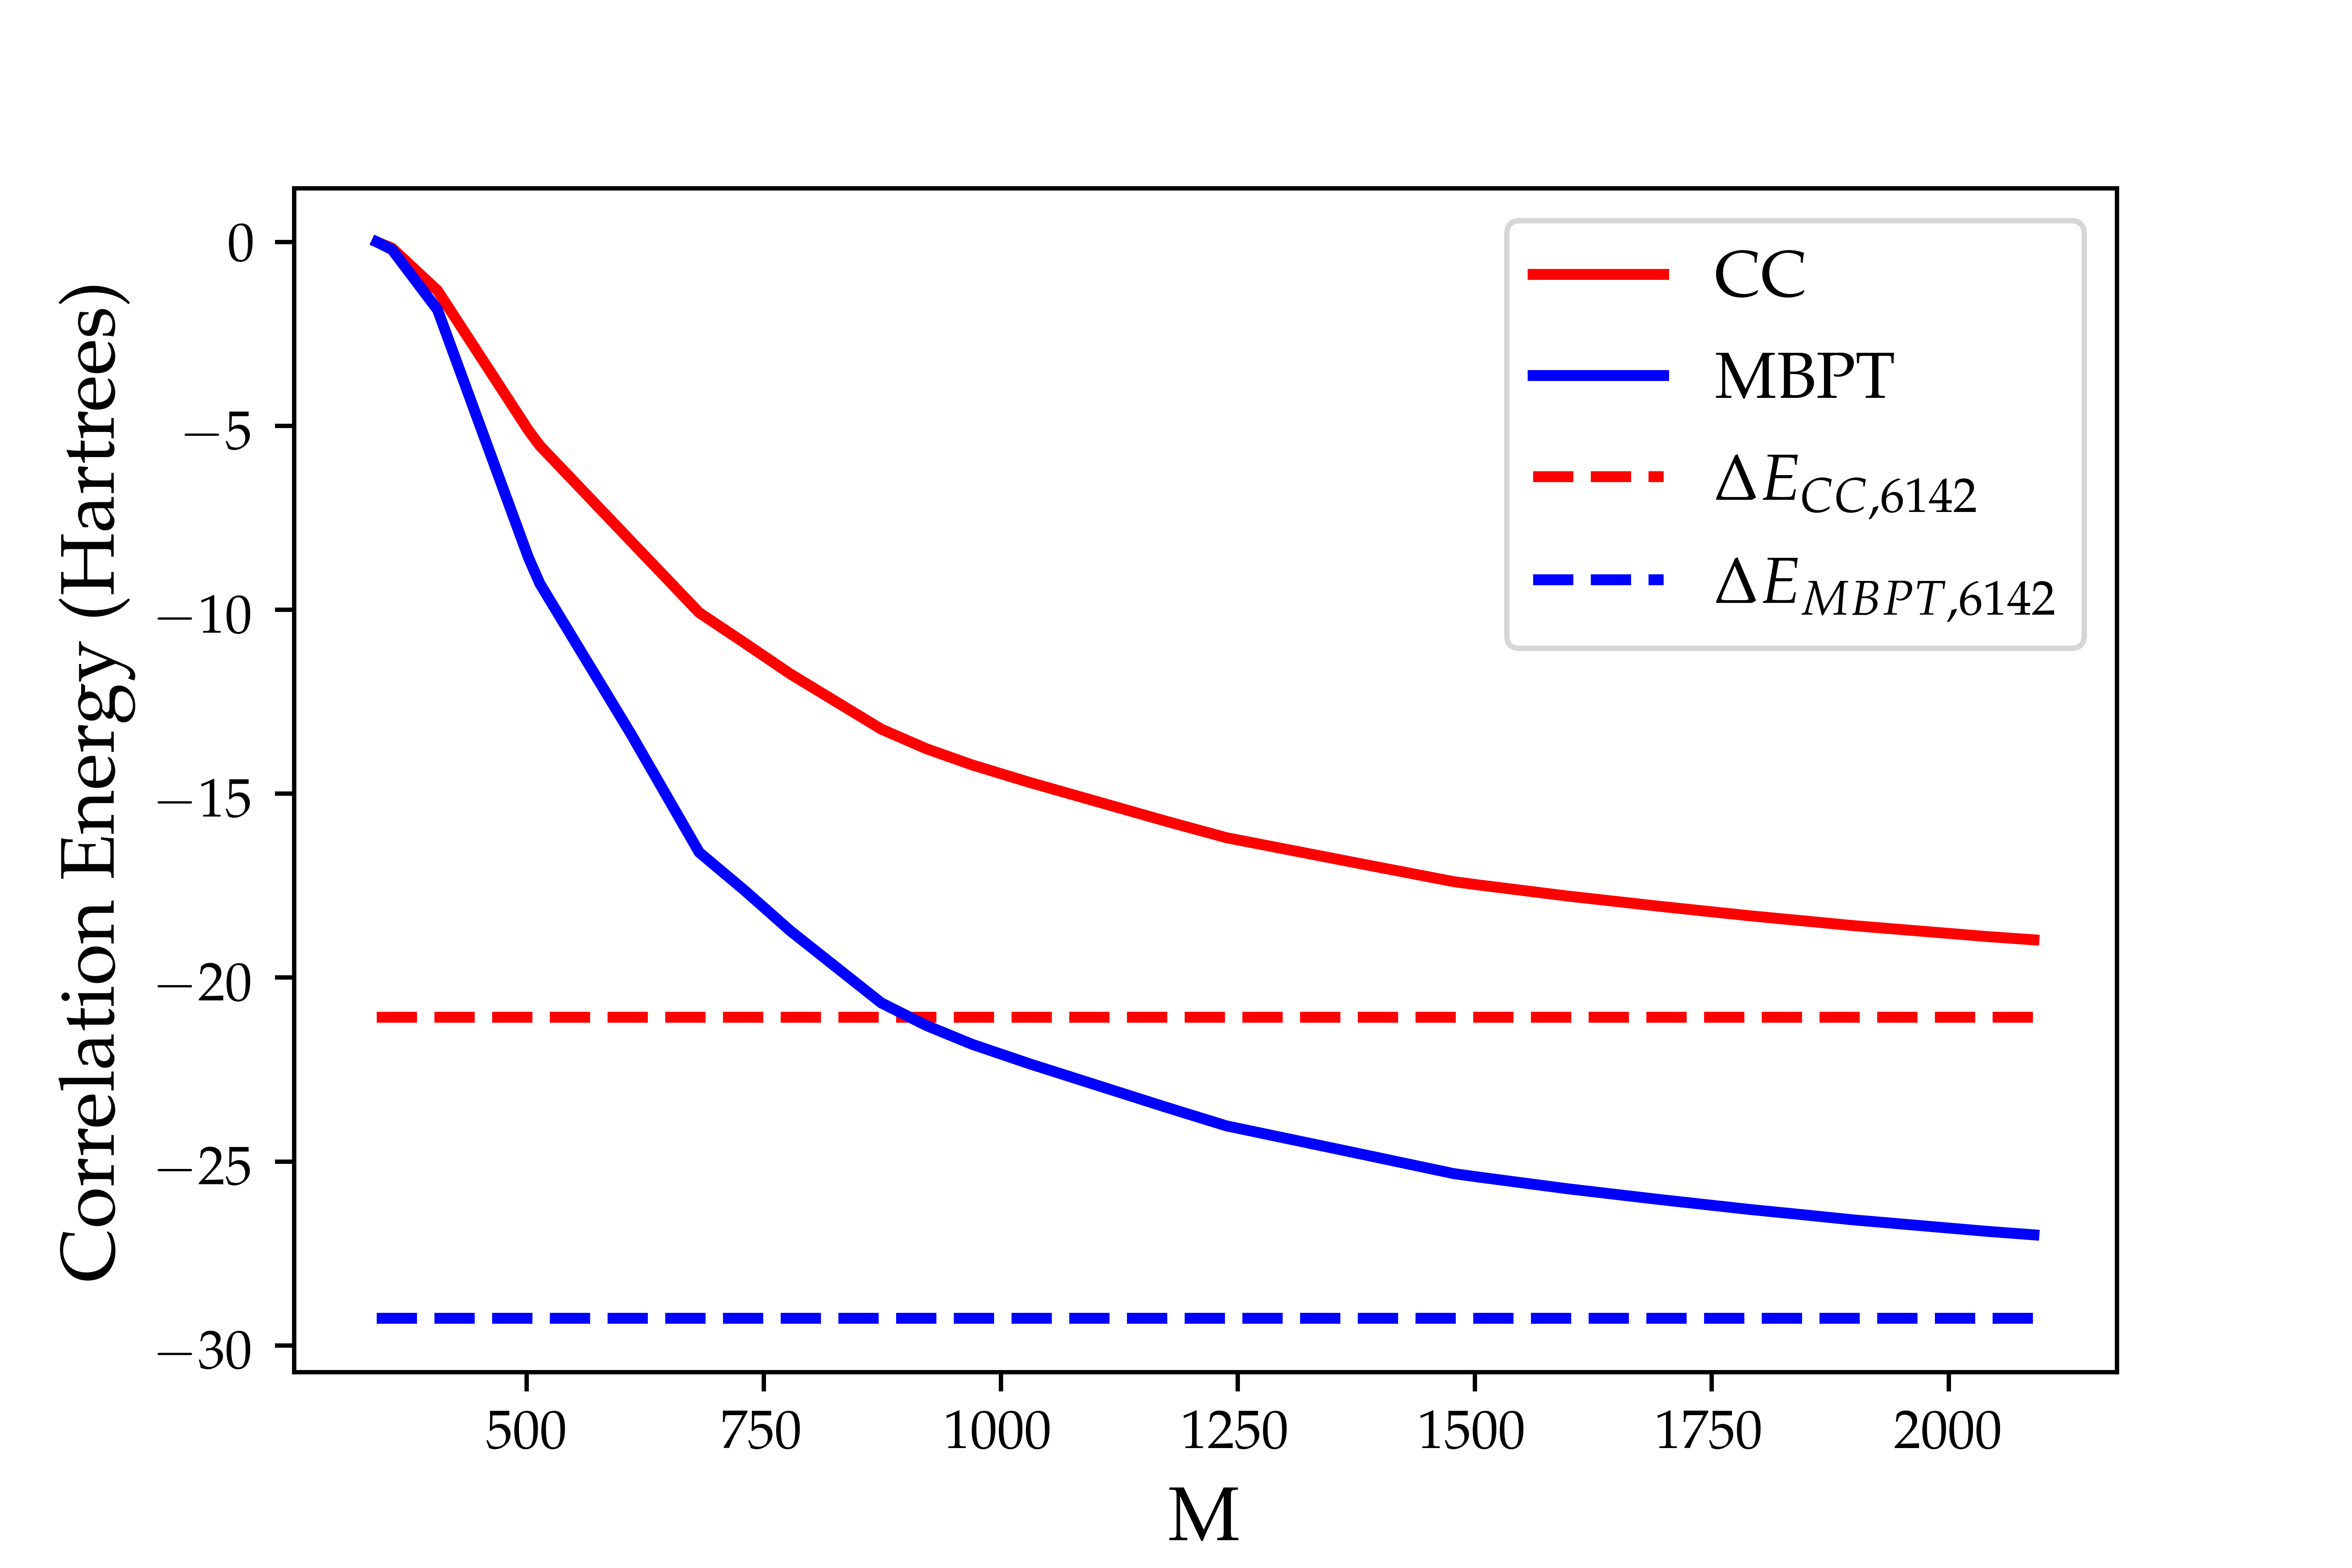
\includegraphics[scale=0.75]{Images/Chapter7/ElectronGas/MBPT_and_CC.png}
    \captionof{figure}{A plot of $\Delta E_{CC}$ and $\Delta E_{MBPT}$ versus M for a HEG system with N=342 and r$_s$=0.5.  The converged correlation energies calculated at M=6142 are shown with dashed lines.}
    \label{mbpt_and_cc}
\end{figure}

Next, we will take Fig. \ref{mbpt_and_cc} and reformat it such that $\Delta E_{CC}$ is plotted as a function of $\Delta E_{MBPT}$ (Fig. \ref{mbpt_vs_cc}).  Each point is at a constant value of M in this format, and M increases from the right to the left. In Fig. \ref{mbpt_vs_cc}, note that the graph is relatively linear, and in fact, it becomes more linear from right to left. Put another way, the graph of $\Delta E_{CC}$ versus $\Delta E_{MBPT}$ becomes more linear as M increases because as M increases, both correlation energies converge. We can check this using Fig. \ref{slopes}

\begin{figure}
    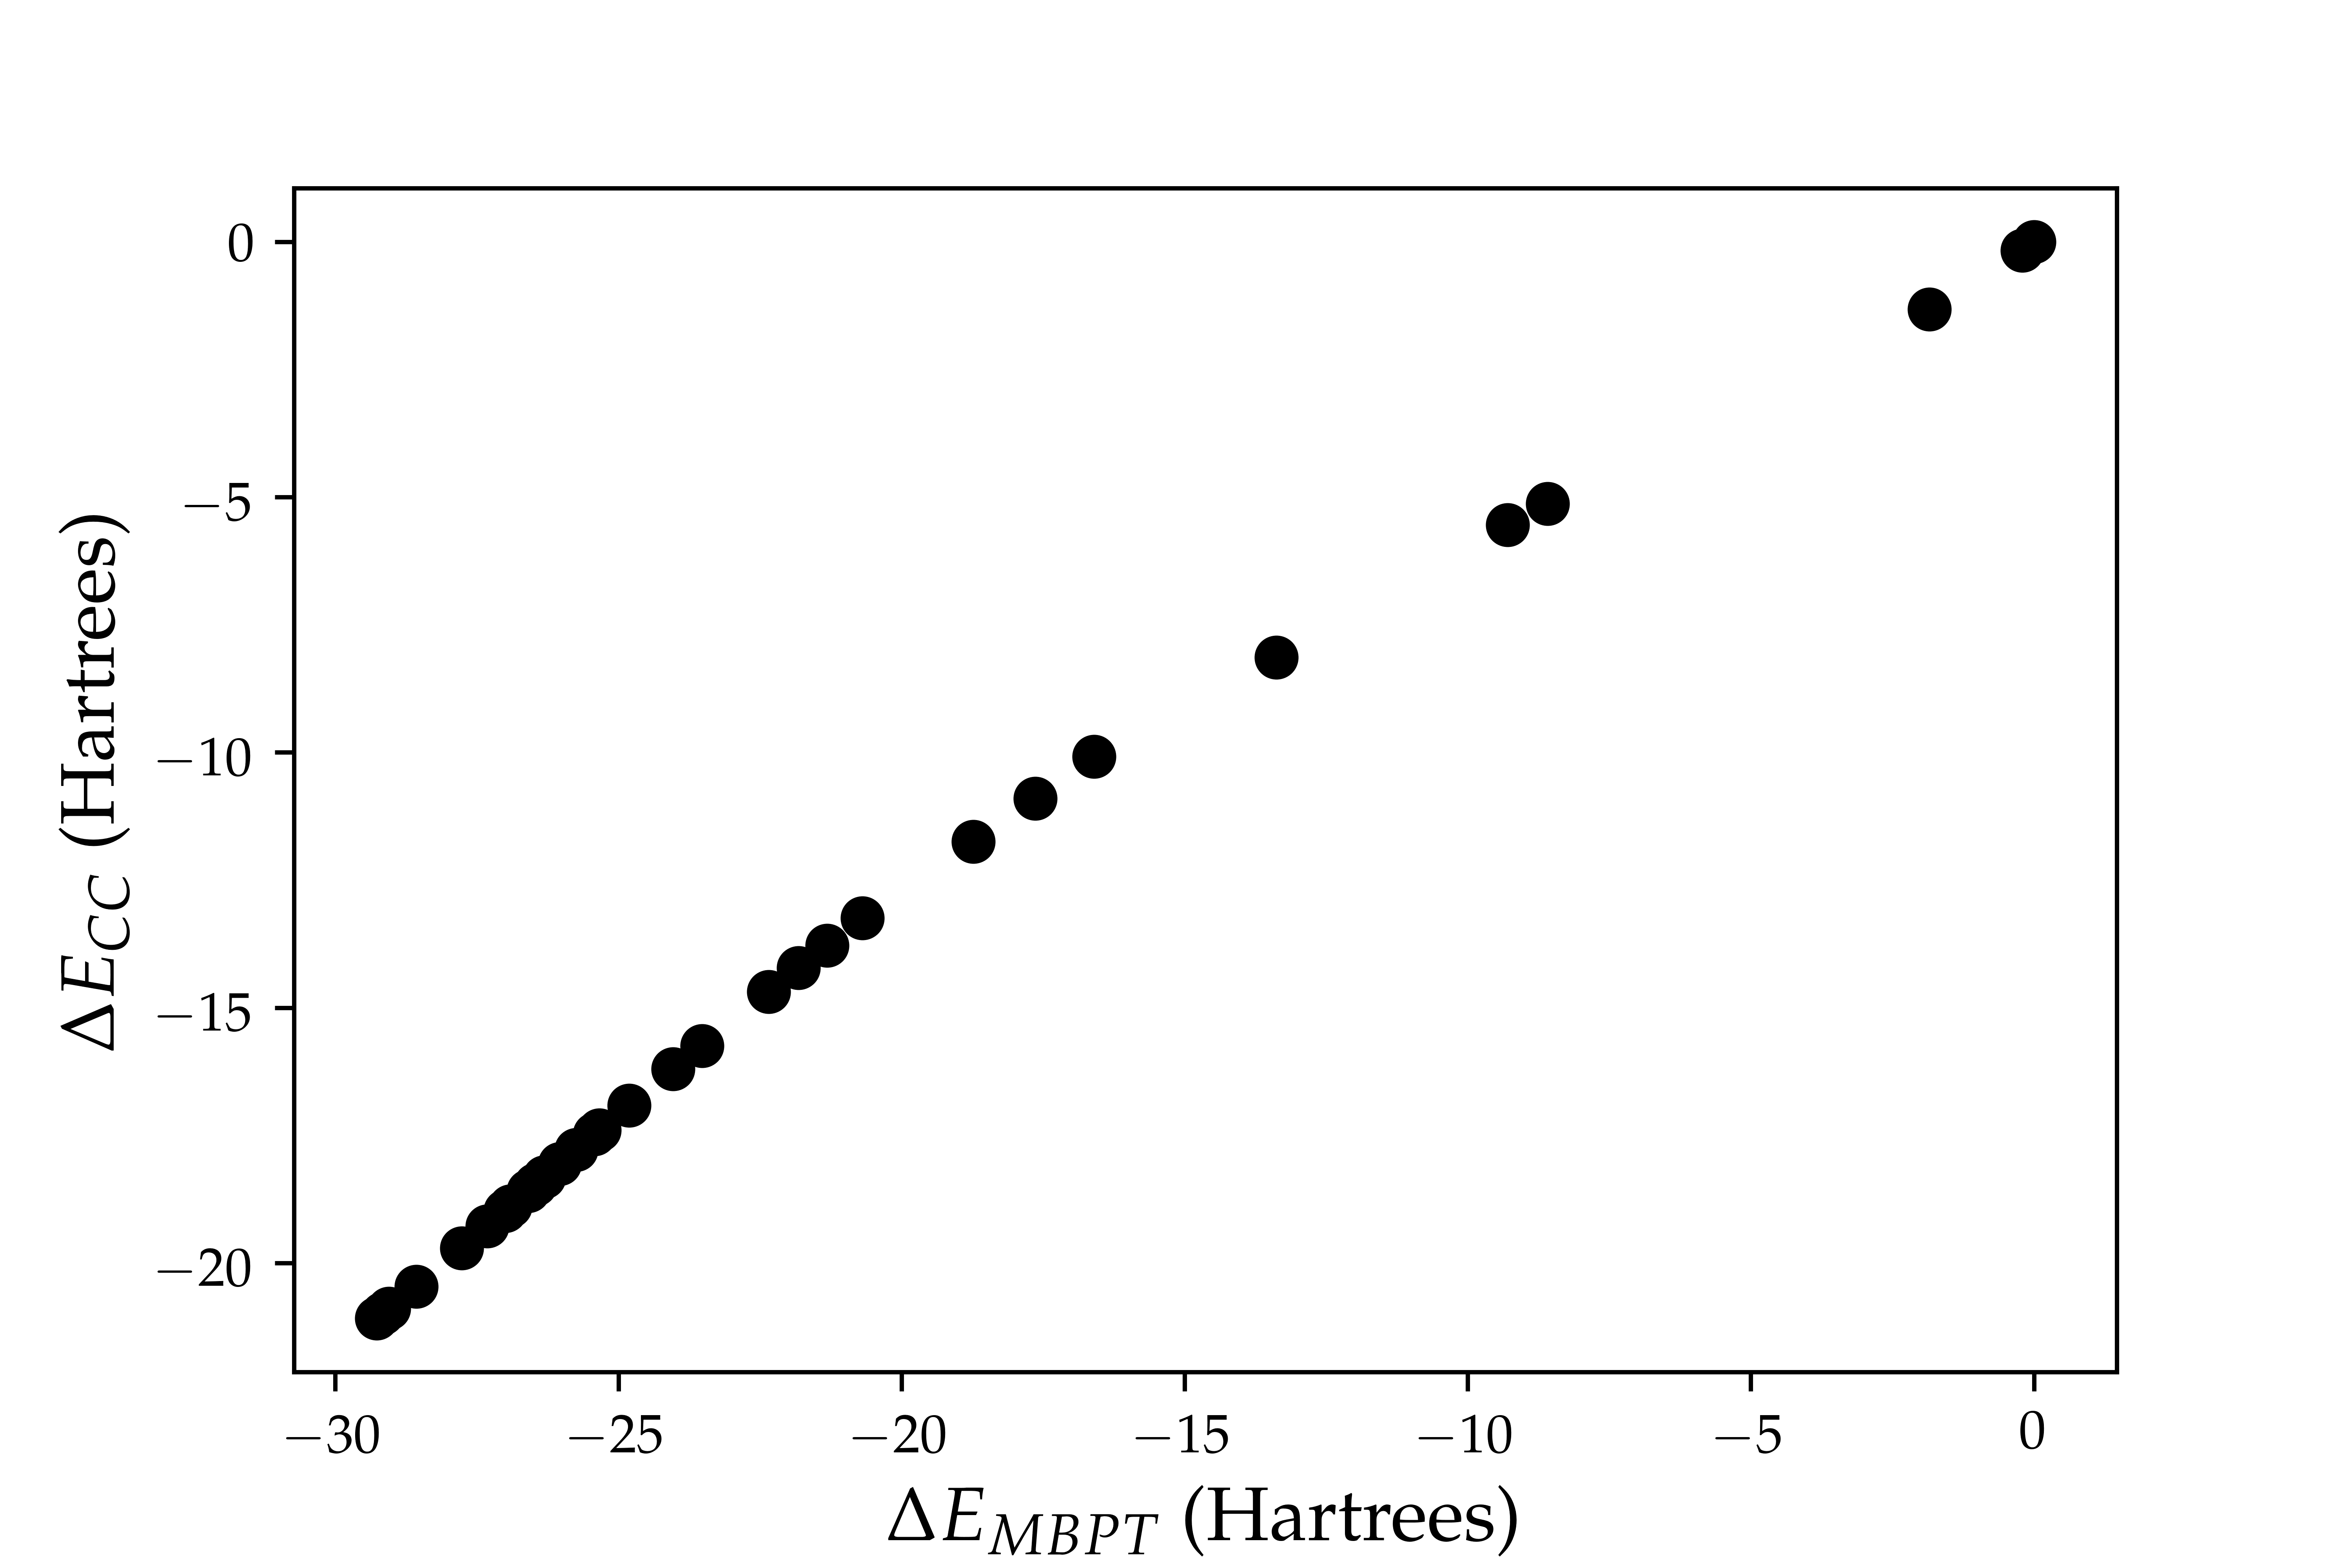
\includegraphics[scale=0.75]{Images/Chapter7/ElectronGas/MBPT_vs_CC.png}
    \captionof{figure}{Figure \ref{mbpt_and_cc} is transformed such that $\Delta E_{CC}$ are plotted as a function of t$\Delta E_{MBPT}$ (such that each point has the same M). The resulting plot has a linear relationship that becomes stronger to the left (as M increases).}
    \label{mbpt_vs_cc}
\end{figure}

Fig. \ref{slopes} shows the ratio of $\Delta E_{CC}$/$\Delta E_{MBPT}$ as a function of the number of single-particle states in the calculations for three different numbers of electrons for calculations of the HEG at $r_s$ = 0.5. The ratio $\Delta E_{CC}$/$\Delta E_{MBPT}$ is the slope of the line in Fig. \ref{mbpt_vs_cc}. While the slopes are rapidly changing at lower values of M, by the end of the graph, all of the slopes are constant, though the slopes at higher numbers of electrons converge slower than the slopes at lower numbers of electrons. However, this graph does verify that the slopes will become constant, and the SRE method should work if we can accurately predict this slope.

\begin{center}
    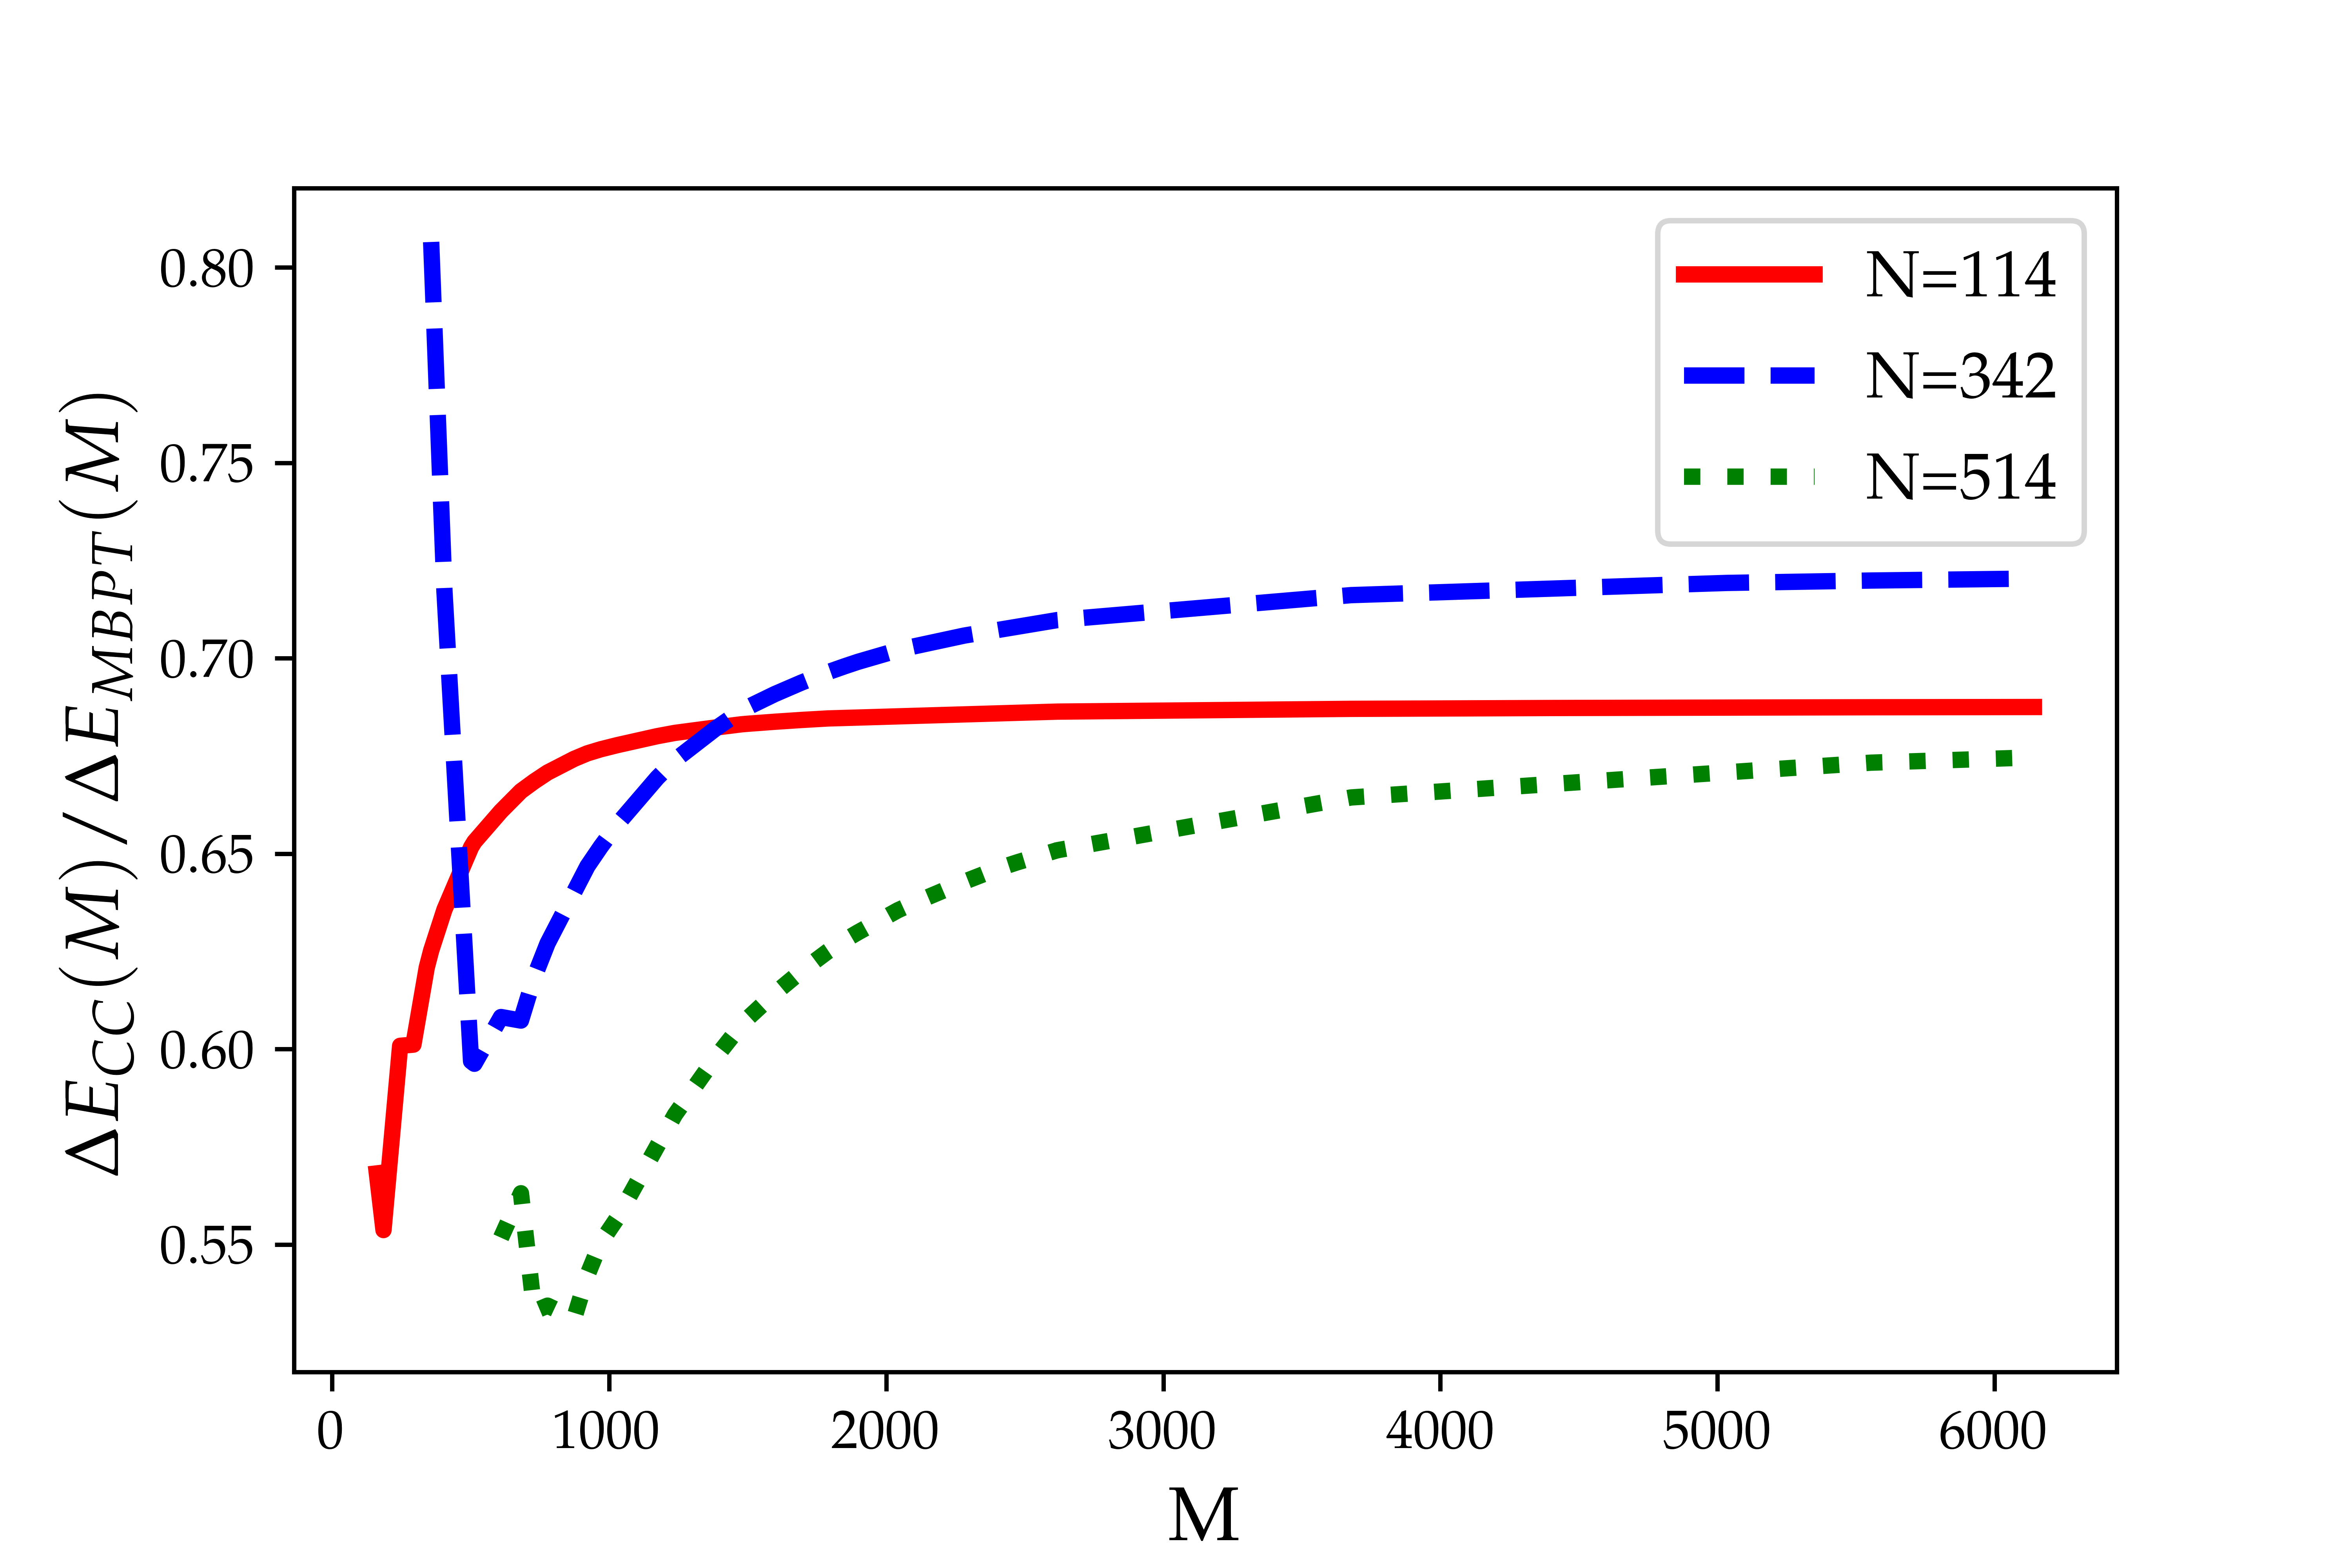
\includegraphics[scale=0.75]{Images/Chapter7/ElectronGas/Slopes.png}
    \captionof{figure}{A plot of the ratio of $\Delta E_{CC}$ to $\Delta E_{MBPT}$ as a function of M for N=114, 342, and 514 and r$_s$=0.5.  As M increases, the ratio (or the slope of the line in Figure FIGURE NUMBER) becomes increasingly constant. However, it is important to note that the run time increases drastically as M increases.}
    \label{slopes}
\end{center}